\begin{frame}
    \frametitle{Sensitivity Analysis with Fuel Cycle Codes}
    \textbf{Motivation for conducting sensitivity analysis}
    \\

    A transition scenario is simulated to predict the 
    future, however when implemented in the real world, 
    it will deviate from the optimal scenario. 
    Therefore, sensitivity analysis studies is necessary to 
    determine how variation in different parameters will impact 
    the progression and final state of the transition scenario. 
    \\

    \textbf{Method}

    Couple fuel cycle codes, \textsc{Cyclus}/DYMOND, 
    with Dakota \cite{eldred_dakota_2010} (sensitivity analysis, 
    optimization, and uncertainty quantification framework).  

    \begin{figure}[]
        \centering
        \begin{tikzpicture}[node distance=2.5cm]
            \tikzstyle{every node}=[font=\large]
            \node (one) [sbblock]{\small Dakota input file};
        \node (two) [bblock, right of=one, xshift = 1cm, text width=3cm]{\tiny Python Script\begin{itemize}
            \item Edit NFC code input file with Dakota's inputs 
            \item Run NFC code with new input file 
            \item Read NFC code database for selected output variable
        \end{itemize}};
        \node  (three) [sbblock, xshift = 1cm, right of=two]{\small Dakota output file};
            
            \draw [arrow] (one) -- (two);
            \draw [arrow] (two) -- (three);
            %\draw [arrow] (three) -- (one);
            %\draw [arrow] (All) -- node[anchor=west] {yes} (End);
            %draw [arrow] (All) -- ([shift={(-3.9cm,0.7cm)}]All.south west)-- node[anchor=east] {no} ([shift={(-3.9cm,-0.85cm)}]Predict.north west)--(Predict);
            \draw [arrow] (three) |-([shift={(0cm,-0.5cm)}]three.south west)-- ([shift={(0cm,-0.5cm)}]one.south east)-|(one);
        \end{tikzpicture}
        \caption{Depiction of coupling of Dakota and NFC code}
        \label{fig:dakota-NFC-flow}
    \end{figure}

\end{frame}
\begin{frame}
    \frametitle{Demand-Driven Cycamore Archetypes Project (NEUP-FY16-10512) }
          \begin{columns}
                  \column[t]{5cm}
                  \textbf{Goal of DDCA Project}
                  \\
                  \vspace{0.1cm} 
                  \begin{itemize}
                      \item Design a \textsc{Cyclus} institution 
                      that will
                      automatically deploy supporting fuel 
                      cycle facilities and reactor 
                      facilities for a user-specified 
                      power demand.
                      \item Demonstrate setting up of 
                      transition scenarios 
                      with undersupply of power. 
                  \end{itemize}
                  \textbf{Progress}
                  \vspace{0.1cm} 
                  \begin{itemize}
                    \item Created \textsc{Cyclus} institution: 
                    \texttt{deploy}
                    \item Set up transition scenarios 
                    (EG01-23/24/29/30 \cite{wigeland_nuclear_2014}) 
                    using \texttt{deploy}
                  \end{itemize}
                  \column[t]{5cm}
          \begin{figure}[htbp!]
          \begin{center}
        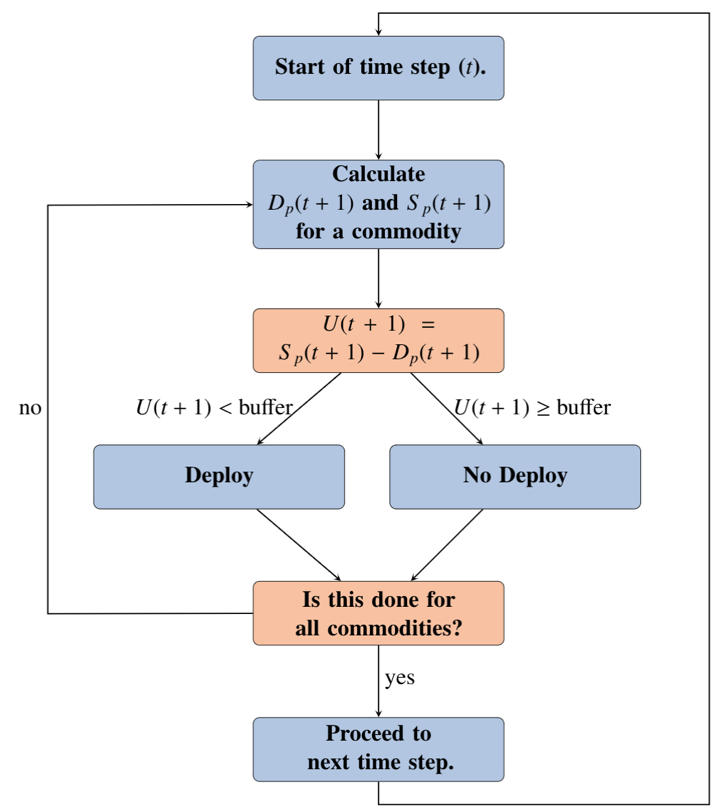
\includegraphics[height=5.5cm]{./images/d3ploy-flow}
      \end{center}
            \caption{\texttt{d3ploy} logic flow \cite{chee_demonstration_2019}}
      \label{fig:d3ploy-flow}
    \end{figure}
          \end{columns}
  \end{frame}
